\documentclass[a4paper,11pt]{article}
\pdfoutput=1 % if your are submitting a pdflatex (i.e. if you have
             % images in pdf, png or jpg format)

\usepackage{jheppub} % for details on the use of the package, please
                     % see the JHEP-author-manual

\usepackage[T1]{fontenc} % if needed



\title{\boldmath A title with some math: $x=1$}


%% %simple case: 2 authors, same institution
%% \author{A. Uthor}
%% \author{and A. Nother Author}
%% \affiliation{Institution,\\Address, Country}

% more complex case: 4 authors, 3 institutions, 2 footnotes
\author[a,b,1]{F. Irst,\note{Corresponding author.}}
\author[c]{S. Econd,}
\author[a,2]{T. Hird\note{Also at Some University.}}
\author[a,2]{and Fourth}

% The "\note" macro will give a warning: "Ignoring empty anchor..."
% you can safely ignore it.

\affiliation[a]{One University,\\some-street, Country}
\affiliation[b]{Another University,\\different-address, Country}
\affiliation[c]{A School for Advanced Studies,\\some-location, Country}

% e-mail addresses: one for each author, in the same order as the authors
\emailAdd{first@one.univ}
\emailAdd{second@asas.edu}
\emailAdd{third@one.univ}
\emailAdd{fourth@one.univ}




\abstract{Abstract...}



\begin{document} 
\maketitle
\flushbottom

\section{Some examples and best-practices}
\label{sec:intro}

For internal references use label-refs: see section~\ref{sec:intro}.
Bibliographic citations can be done with cite: refs.~\cite{a,b,c}.
When possible, align equations on the equal sign. The package
\texttt{amsmath} is already loaded. See \eqref{eq:x}.
\begin{equation}
\label{eq:x}
\begin{split}
x &= 1 \,,
\qquad
y = 2 \,,
\\
z &= 3 \,.
\end{split}
\end{equation}
Also, watch out for the punctuation at the end of the equations.


If you want some equations without the tag (number), please use the available
starred-environments. For example:
\begin{equation*}
x = 1
\end{equation*}

The amsmath package has many features. For example, you can use use
\texttt{subequations} environment:
\begin{subequations}\label{eq:y}
\begin{align}
\label{eq:y:1}
a & = 1
\\
\label{eq:y:2}
b & = 2
\end{align}
and it will continue to operate across the text also.
\begin{equation}
\label{eq:y:3}
c = 3
\end{equation}
\end{subequations}
The references will work as you'd expect: \eqref{eq:y:1},
\eqref{eq:y:2} and \eqref{eq:y:3} are all part of \eqref{eq:y}.

A similar solution is available for figures via the \texttt{subfigure}
package (not loaded by default and not shown here). 
All figures and tables should be referenced in the text and should be
placed at the top of the page where they are first cited or in
subsequent pages. Positioning them in the source file
after the paragraph where you first reference them usually yield good
results. See figure~\ref{fig:i} and table~\ref{tab:i}.

\begin{figure}[tbp]
\centering % \begin{center}/\end{center} takes some additional vertical space
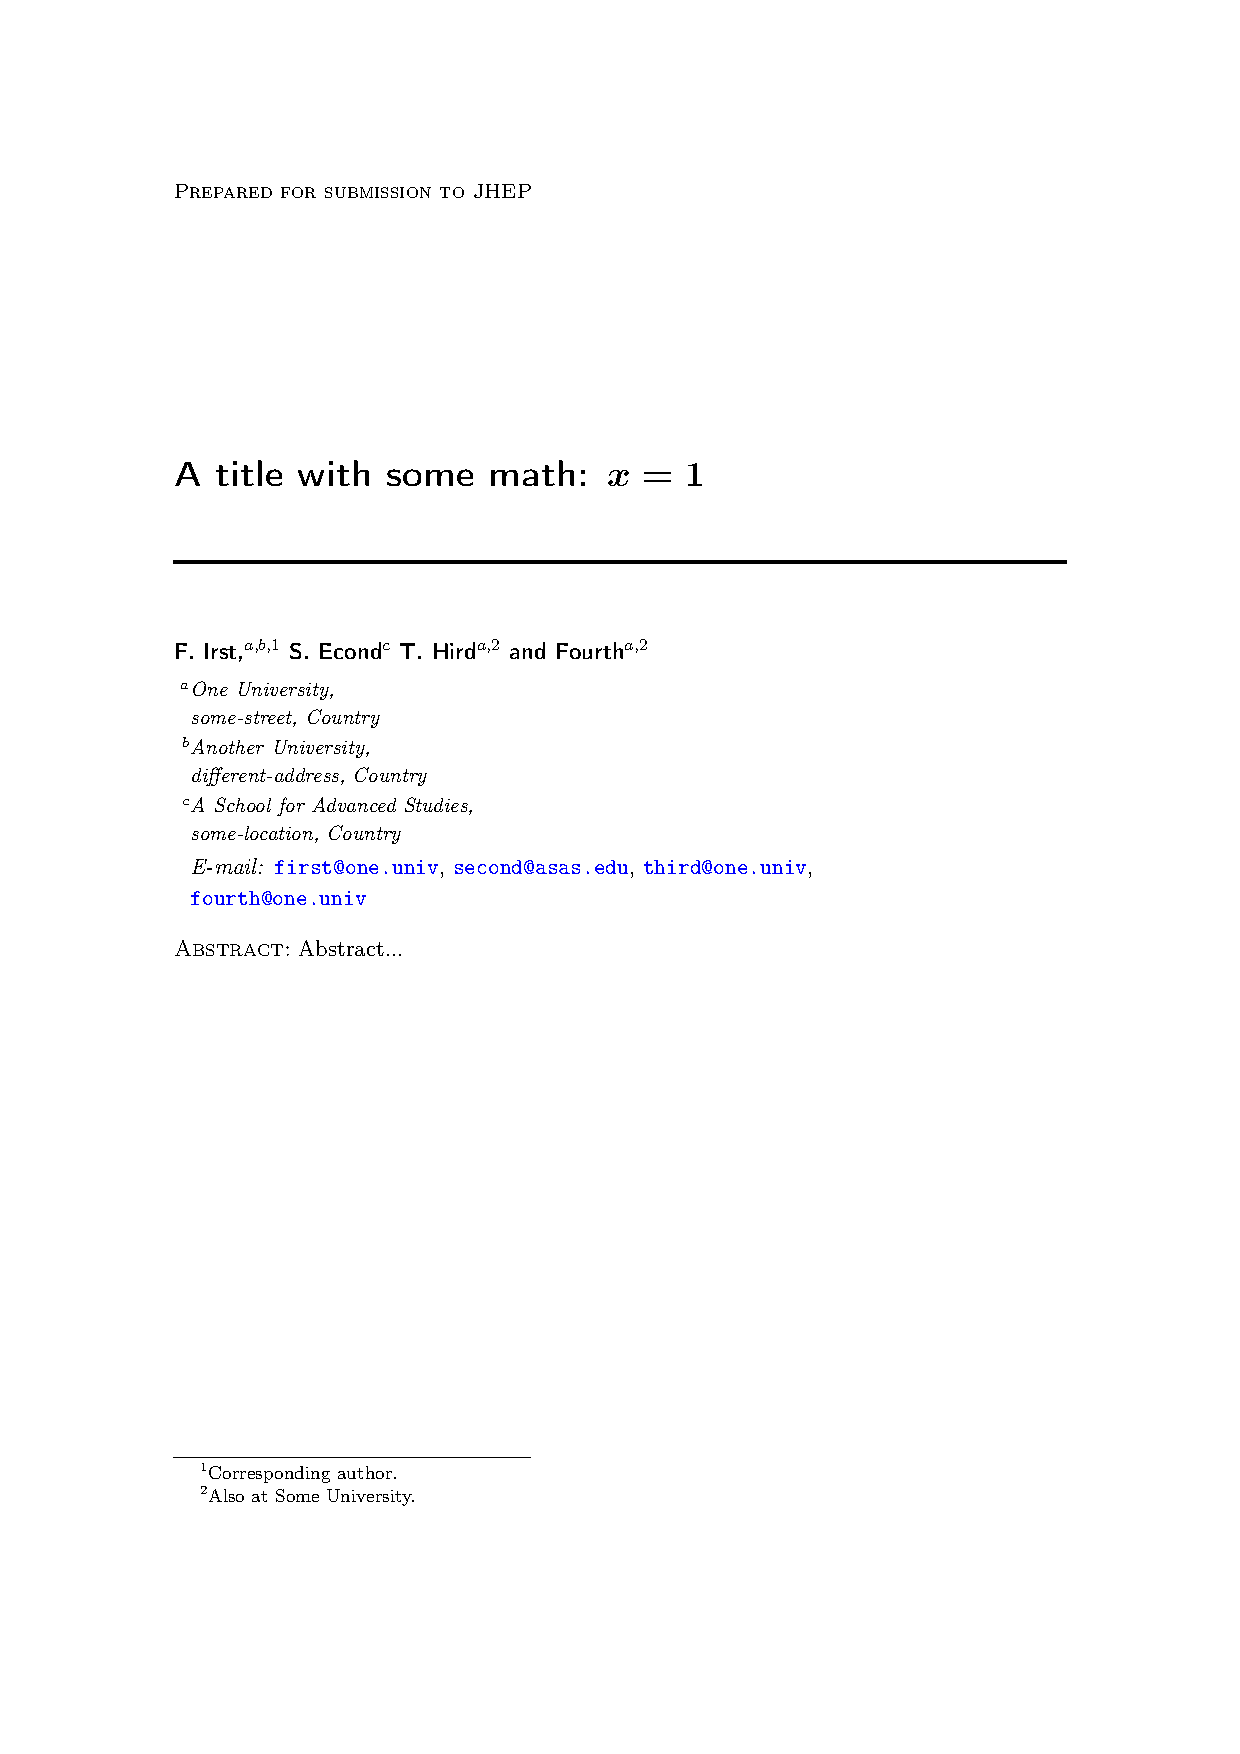
\includegraphics[width=.45\textwidth,trim=0 380 0 200,clip]{img1.pdf}
\hfill
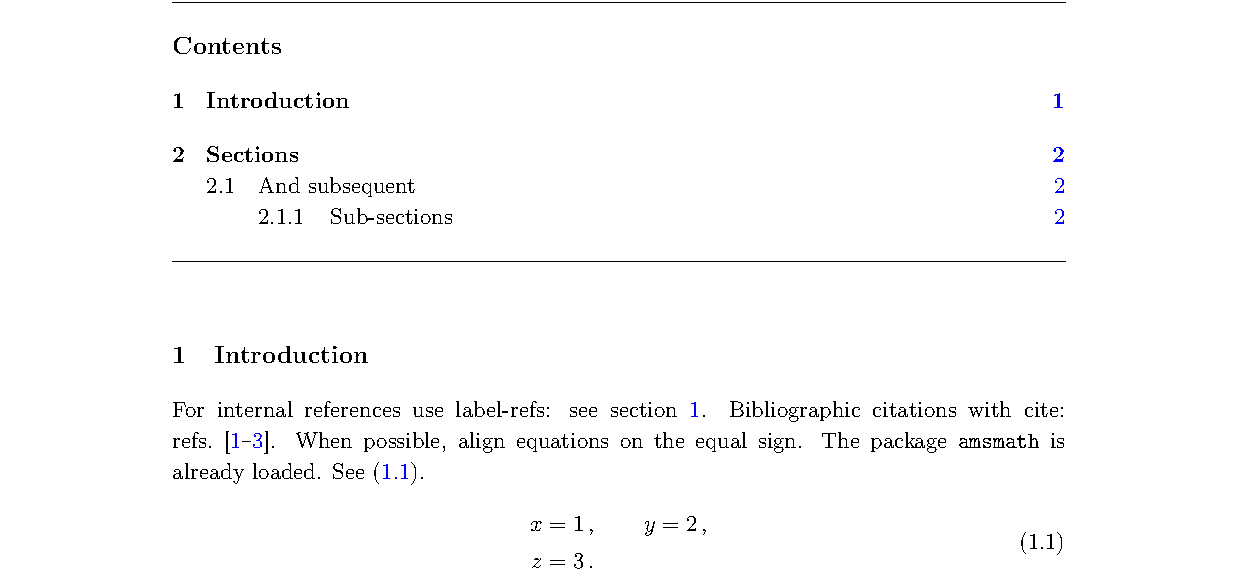
\includegraphics[width=.45\textwidth,origin=c,angle=180]{img2.pdf}
% "\includegraphics" is very powerful; the graphicx package is already loaded
\caption{\label{fig:i} Always give a caption.}
\end{figure}

\begin{table}[tbp]
\centering
\begin{tabular}{|lr|c|}
\hline
x&y&x and y\\
\hline 
a & b & a and b\\
1 & 2 & 1 and 2\\
$\alpha$ & $\beta$ & $\alpha$ and $\beta$\\
\hline
\end{tabular}
\caption{\label{tab:i} We prefer to have borders around the tables.}
\end{table}

We discourage the use of inline figures (wrapfigure), as they may be
difficult to position if the page layout changes.

We suggest not to abbreviate: ``section'', ``appendix'', ``figure''
and ``table'', but ``eq.'' and ``ref.'' are welcome. Also, please do
not use \texttt{\textbackslash emph} or \texttt{\textbackslash it} for
latin abbreviaitons: i.e., et al., e.g., vs., etc.



\section{Sections}
\subsection{And subsequent}
\subsubsection{Sub-sections}
\paragraph{Up to paragraphs.} We find that having more levels usually
reduces the clarity of the article. Also, we strongly discourage the
use of non-numbered sections (e.g.~\texttt{\textbackslash
  subsubsection*}).  Please also see the use of
``\texttt{\textbackslash texorpdfstring\{\}\{\}}'' to avoid warnings
from the hyperref package when you have math in the section titles



\appendix
\section{Some title}
Please always give a title also for appendices.





\acknowledgments

This is the most common positions for acknowledgments. A macro is
available to maintain the same layout and spelling of the heading.

\paragraph{Note added.} This is also a good position for notes added
after the paper has been written.





% The bibliography will probably be heavily edited during typesetting.
% We'll parse it and, using the arxiv number or the journal data, will
% query inspire, trying to verify the data (this will probalby spot
% eventual typos) and retrive the document DOI and eventual errata.
% We however suggest to always provide author, title and journal data:
% in short all the informations that clearly identify a document.

\begin{thebibliography}{99}

\bibitem{a}
Author, \emph{Title}, \emph{J. Abbrev.} {\bf vol} (year) pg.

\bibitem{b}
Author, \emph{Title},
arxiv:1234.5678.

\bibitem{c}
Author, \emph{Title},
Publisher (year).


% Please avoid comments such as "For a review'', "For some examples",
% "and references therein" or move them in the text. In general,
% please leave only references in the bibliography and move all
% accessory text in footnotes.

% Also, please have only one work for each \bibitem.


\end{thebibliography}
\end{document}
